\section{Experiment}
\label{sec:experiment}
%
The simulation experiments we run in Gymnasium supports the theoretical
computation performed in Section~\ref{ssec:prob_sol}. The Monte Carlo
simulations that we perform can yield even more results, such as what is the 
expected number of ``bad'' moves that the robot makes before it reaches the goal. Here, a bad move means that the agent moves away from the goal. We can 
further compute a histogram of the states visited, and the rewards collected on 
average.

The first result in Figure~\ref{fig:running_avg} shows the running average
number of steps taken to reach the goal over $50,000$ independent Monte Carlo
simulation runs.
%
\begin{figure}[tb]
    \centering
    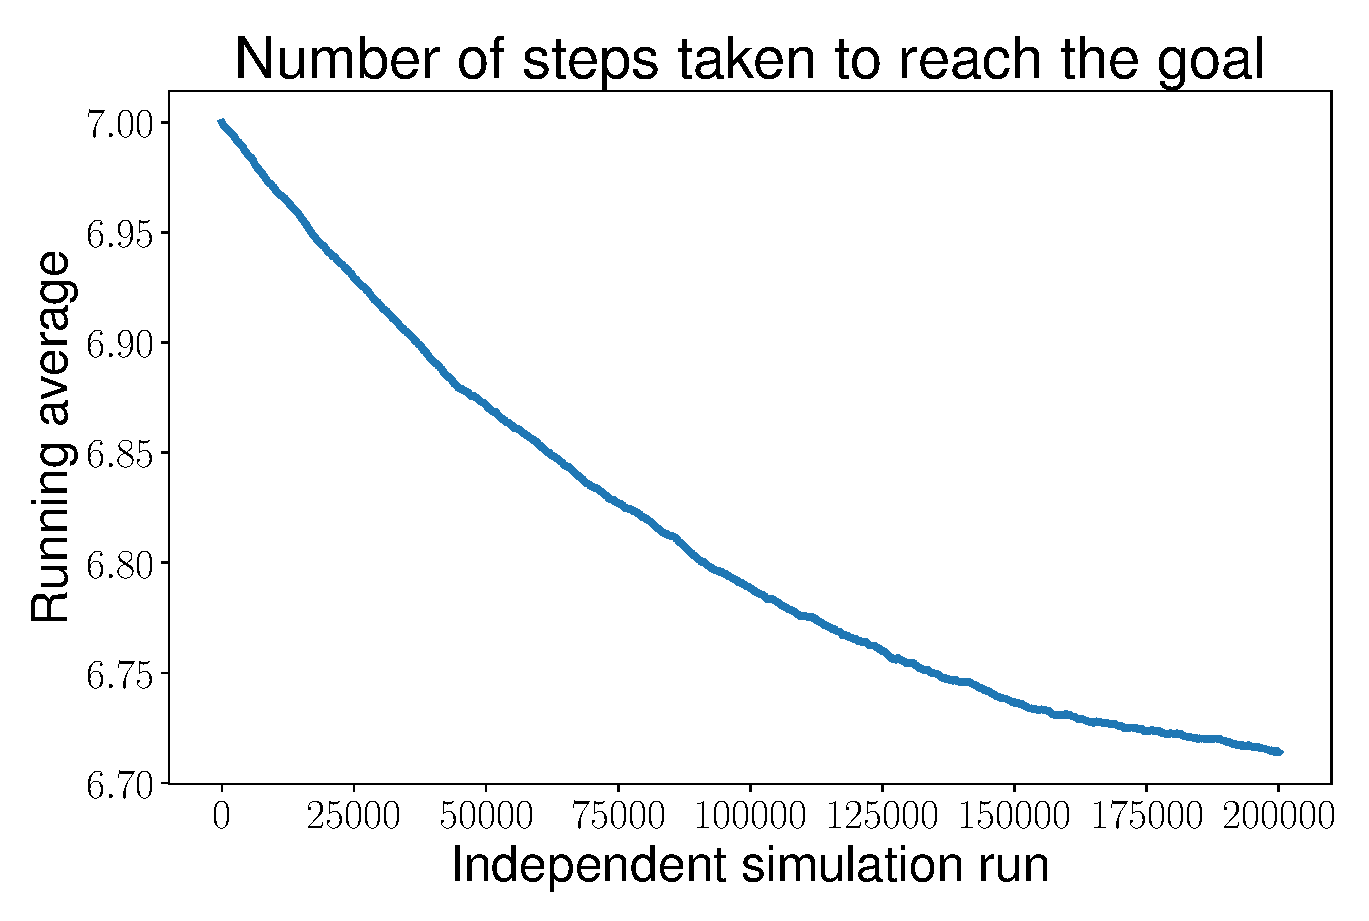
\includegraphics[width=0.5\textwidth]{./figures/running_avg.eps}
    \caption{Running average number of steps taken to reach the goal over $50,000$ independent Monte Carlo simulation runs.}
    \label{fig:running_avg}
\end{figure}
%
Figure~\ref{fig:running_avg} shows that the running average converges to $6.\bar{6}$ just as the theoretical computation indicated in Section~\ref{ssec:prob_sol}.

Table~\ref{tab:histogram} contains the probabilities of number of steps it took
to solve the environment over $50,000$ independent Monte Carlo simulation runs.
These probabilities are calculated empirically by counting the number of times
the agent takes $4$, $6$, and $8$ steps to reach the goal and dividing by the
total number of runs. We observe that it takes $4$ steps to solve the
environment $16.\bar{6}\%$ of the time, $6$ steps $33.\bar{3}\%$ of the time,
and $8$ steps $50\%$ of the time, yielding an expected value of 
%
\[
\frac{1}{6} \times 4 + \frac{1}{3} \times 6 + \frac{1}{2} \times 8 = \frac{20}{3} = 6.\bar{6}.
\]
%
% \begin{figure}[bt]
%     \centering
%     \includegraphics[width=0.48\textwidth]{./figures/steps_histogram.eps}
%     \caption{Histogram of number of steps taken to solve the environment over $50,000$ independent Monte Carlo simulation runs.}
%     \label{fig:histogram}
% \end{figure}
%
\begin{table}[b]
    \caption{Histogram of the number of steps taken to solve the environment 
    over $50,000$ Monte Carlo simulation runs.}
    \label{tab:histogram}
    \centering
    \begin{tabular}{*4l} \toprule
        \textit{Probability} & $\nicefrac{1}{6}$ & $\nicefrac{1}{3}$ & $\nicefrac{1}{2}$ \\
        \textit{Steps} & $4$ & $6$ & $8$ \\
    \bottomrule
    \hline
    \end{tabular}
\end{table}
%
The shorter the path the agent takes to reach the goal, the more uncertain it
tends to be about the identity of the true world. For instance, if it takes only
$4$ steps to reach the goal, the agent may only know that the world might be 
$1$ of the $12$ possible worlds, having eliminated the remaining $12$. However, 
if it takes $8$ steps to reach the goal, it will have eliminated $20$ of the 
possible $24$ worlds that it starts with and is certain that the true world is 
one of the remaining $4$. If the agent takes $6$ steps to solve the environment,
then it may only have eliminated $14$ of $24$, still remaining with $10$ possible worlds. Notice that this doesn't mean that the agent cannot solve the 
environment; indeed, it still can and has.

Figure~\ref{fig:visit_count} shows the frequency of visits of each state under
the optimal policy deduced by $Q$-learning over $50,000$ independent Monte Carlo
runs. Notice that the ratio of the goal state being visited to the number of
runs is $1$, meaning that all runs end at the goal state. Further, we see that
the states the robot passes through either $(4, 2)$ or $(2, 4)$ to reach the
goal, and never through $(3, 3)$. The reason that this happens is that the $Q$-
learning algorithm acts greedily with respect to its value estimates and when 
the agent reaches one of the states $(3, 2)$ or $(2, 3)$, it will always value 
the action it took to get there more than the others; hence continuing on to 
$(4, 2)$ or $(2, 4)$, respectively, instead of trying out the state $(3, 3)$.
%
\begin{figure}[tb]
    \centering
    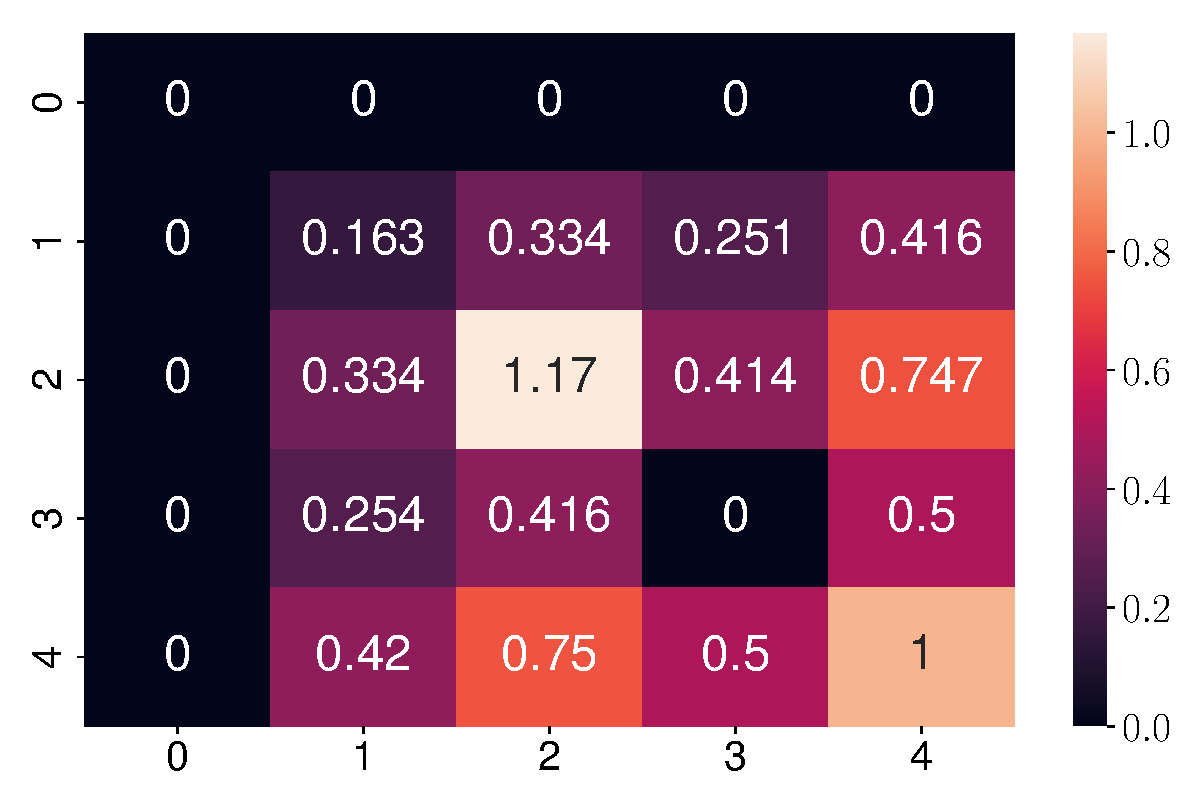
\includegraphics[width=0.48\textwidth]{./figures/visit_count_ratio.eps}
    \caption{Ratio of times a given state is visited under the optimal policy to the number $50,000$ of independent Monte Carlo simulation runs.}
    \label{fig:visit_count}
\end{figure}

Figure~\ref{fig:bandit_scores} shows the scores each world belief achieves over
simulation steps during a single run that lasts $8$ steps. At the end there are
four bandit arms (world beliefs) that have the same high score of $1$, however,
two of these bandits arms have been identified to swap the ``down'' and
``right'' actions. Since this swapping does not affect the performance of the
agent, their score matches the other two top bandit arms which have not been
differentiated.
%
\begin{figure}[bt]
    \centering
    \includegraphics[width=0.48\textwidth]{./figures/bandit_scores.eps}
    \caption{Smoothed scores each world belief achieves over a single run sample.}
    \label{fig:bandit_scores}
\end{figure}